% Census, calibration and manipulation check. Outcome-independent: every number here comes from
% results/predictions.json (sha 16f9e895...), written before any outcome run, and from the on-device
% displacement traces of the tuning runs (studies/S1/manipulation_B11.json).
\subsection{Census, calibration and manipulation check}\label{sec:census}

\paragraph{Concentration}
The census covers 24{,}576 eval-mode rows of the pretrained encoder (2{,}048 per layer) and 49{,}152 rows of
the reference language model, pooled over four training snapshots. Encoder attention is much more
concentrated. The mean top-4 mass $A_4$ is 0.46 in the encoder and 0.21 in the LM, the median is 0.45 and 0.13,
and the mean $\mathrm{TV}(a,u)$ is 0.72 and 0.28. Across encoder rows, $A_4$ ranges from 0.069 at the 5th
percentile to 0.97 at the 95th. At $p=0.1$ and $k=4$ the dispersion index $\kappa=\mathbb E m^2/\mathbb E m$ is
0.318 in the encoder and 0.172 in the LM. The exploratory premise $\kappa_E\ge2\kappa_L$ from the protocol
therefore does not hold (0.318 versus 0.344).

\paragraph{Operating points}
Table~\ref{tab:calib} lists the calibrated parameters at $\ell=0.10$ with the exact displacement moments
implied by the census. The nominal parameters needed to reach the same mean displacement differ widely
between families. The Relaxed Attention coefficient is 0.14 in the encoder and 0.36 in the LM, and the
unbudgeted top-4 deletion rate is 0.22 and 0.49. This is Proposition~\ref{prop:laws} at work: a single nominal
rate would deliver different doses in the two regimes. Within the deletion class of
Proposition~\ref{thm:cx}, the ordering $S_2^{\mathrm{HB}}<S_2^{\mathrm{HF}}<S_2^{\mathrm{HU}}$ holds in both
regimes, as it must. CapDrop's second moment is 62\% (encoder) and 61\% (LM) of the fixed-$\alpha$ arm's. The cap binds on 54\% and 32\% of rows. The registered separation
$\delta=(S_2^{\mathrm{HF}}-S_2^{\mathrm{HB}})/\ell^2$ is 0.75 in the encoder and 0.83 in the LM. Both exceed the
prespecified threshold $c=0.5$. The registered expectations are therefore ``HB better'' for H1-E and ``HB not better
(equivalent or worse)'' for H1-L; both tests remain two-sided. An earlier protocol rule would have
registered H1-L as ``equivalent'' because the LM's median $A_4$ is below 0.2. That rule was replaced before the
freeze, and the replacement expectation includes equivalence. At $\ell=0.20$ no deletion arm reaches the level in the LM:
even at $p=1$, $\mathbb E m=0.1997$. The three deletion arms run at $p=1$ with no effective cap there, so they coincide and are run once.

Figure~\ref{fig:census} shows what the matched mean hides. At the same pooled mean of 0.10, unbudgeted and
fixed-$\alpha$ deletion leave a long tail. In the encoder, 1.3\% of HU draws displace a row by more than 0.8, and HF displacements reach 0.43.
CapDrop's displacement stops at $\tau$. Calibration pools layers, so the dose still differs between layers. Across
the encoder's layers it ranges from 0.041 to 0.151 for HU and HF, whose per-layer means coincide by construction,
and from 0.056 to 0.123 for CapDrop. The cap binds on 17\% of rows in the first layer and on 80\% in the last.

\begin{figure}[t]
\centering
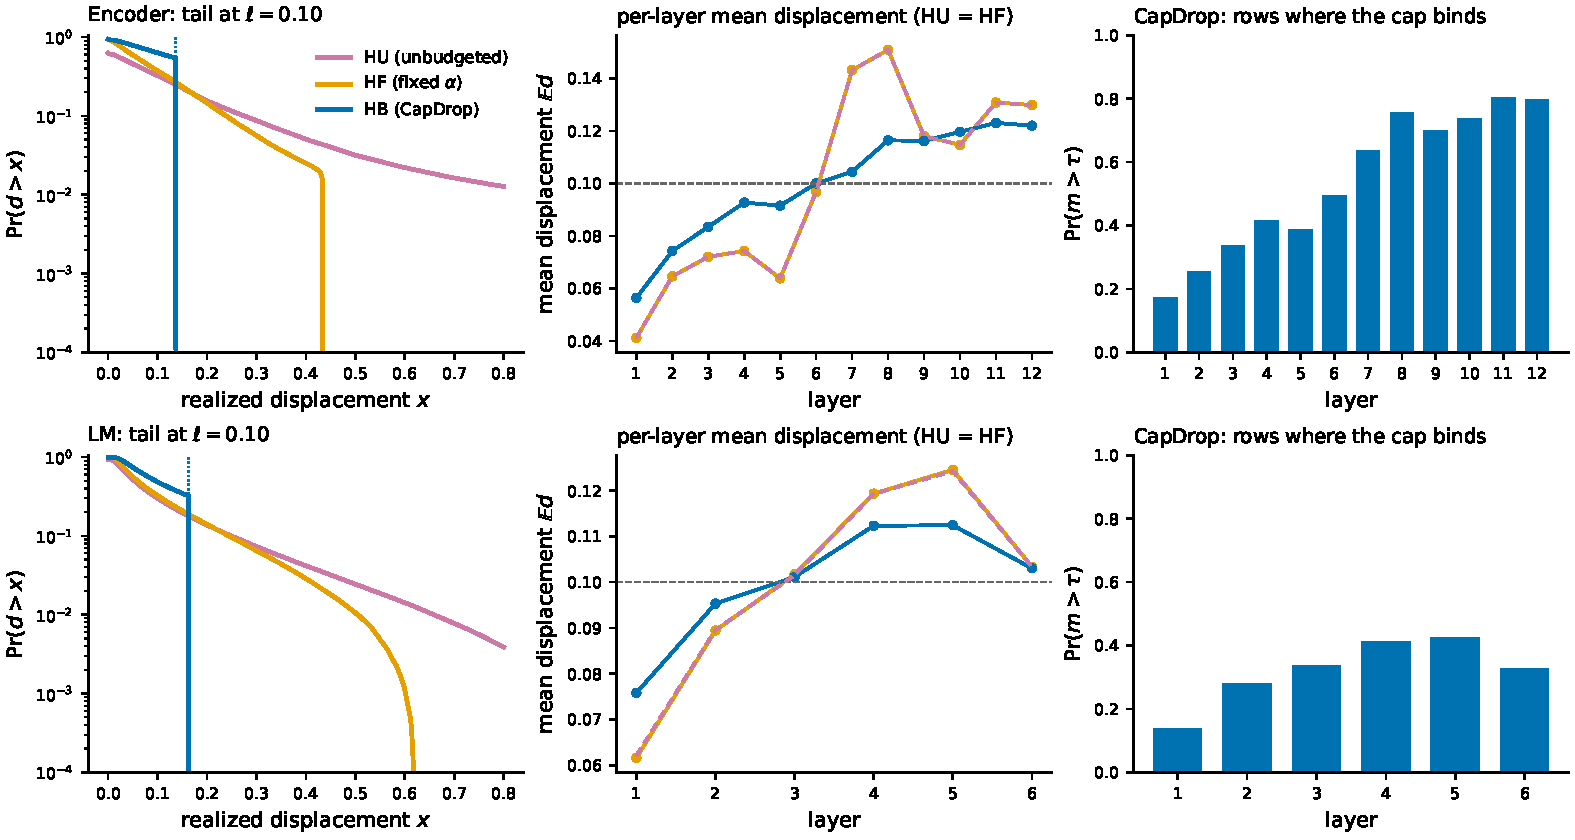
\includegraphics[width=\linewidth]{figures/fig_census.pdf}
\caption{Displacement at matched mean $\ell=0.10$ on the census rows (exact over all 16 deletion patterns of every
row; before any outcome). Left: survival function of the realized displacement $d$. Middle: mean displacement
per layer; the calibration target is the pooled mean (dashed). Right: fraction of rows on which CapDrop's cap binds.
Top: pretrained BiomedBERT; bottom: reference language model.}
\label{fig:census}
\end{figure}

\begin{table}[t]
\centering
\caption{Calibrated operating points at mean displacement $\ell=0.10$ (census, before any outcome). $S_2=\mathbb E d^2$,
$B$ is the train/evaluation mean shift and $\Pr(m>\tau)$ the fraction of rows on which the cap binds. DK uses
DropKey's linear depth schedule (maximum rate shown); its mean shift is not available in closed form.}
\label{tab:calib}
\footnotesize
\setlength{\tabcolsep}{2.6pt}
\begin{tabular}{llcccclccc}
\toprule
& & \multicolumn{4}{c}{Encoder (BiomedBERT)} & & \multicolumn{3}{c}{LM (from scratch)}\\
\cmidrule{3-6}\cmidrule{8-10}
Arm & Parameter & value & $S_2\times10^{2}$ & $B$ & $\Pr(m>\tau)$ & & value & $S_2\times10^{2}$ & $B$\\
\midrule
AD & $p$ & 0.100 & 1.25 & 0 & -- & & 0.100 & 1.08 & 0\\
DK & $p_{\max}$ & 0.185 & 2.42 & -- & -- & & 0.172 & 1.57 & --\\
RA & $\gamma$ & 0.138 & 1.09 & 0.100 & -- & & 0.361 & 1.44 & 0.100\\
RB & $\tau$ & 0.100 & 1.00 & 0.100 & -- & & 0.104 & 1.01 & 0.100\\
HU & $p$ & 0.217 & 3.59 & 0.062 & -- & & 0.491 & 2.69 & 0.079\\
HF & $p$, $\gamma$ & 0.5, 0.434 & 1.99 & 0.072 & -- & & 0.8, 0.620 & 2.12 & 0.090\\
HB & $p$, $\tau$ & 0.5, 0.137 & 1.24 & 0.070 & 0.54 & & 0.8, 0.163 & 1.29 & 0.092\\
\midrule
\multicolumn{2}{l}{$\delta=(S_2^{\mathrm{HF}}-S_2^{\mathrm{HB}})/\ell^2$} & \multicolumn{4}{c}{0.75} & & \multicolumn{3}{c}{0.83}\\
\bottomrule
\end{tabular}
\end{table}

\paragraph{Does displacement reach the head output?}
A registered value-weighted census checks whether the realized displacement of a row predicts how far the head
output moves. It is computed exactly for the top-4 deletion arms by enumerating all 16 deletion patterns, and with 64
Monte Carlo draws for AD and DK. Pooled over families at $\ell=0.10$, the Spearman correlation between $d$ and
$\lVert\Delta z\rVert$ is 0.54 in the encoder and 0.67 in the LM. Both are above the registered refutation
threshold of 0.5, so the premise of displacement accounting is not refuted, though in the encoder the margin is small.
The correlation is high for the deletion arms (0.51--0.90 in the encoder, 0.75--0.95 in the LM). It is low for
attention dropout (0.14 and 0.24), whose rows are not normalized. For TV-budgeted relaxation it is near zero,
because its displacement is almost constant. The mean relative change of the head output is 0.11--0.15 in the encoder.
The protocol also registered a secondary prediction: that the cap lowers the share of deleted mass that falls on special tokens.
This holds in the LM (1.6\% for HB versus 2.4\% for HF) but not in the encoder (16.5\% versus 14.2\%).
In the LM the value census uses the final checkpoint, whose attention is more concentrated than
the pooled calibration census. There, the arms whose displacement depends on concentration (RA and the top-4
deletion arms) have a realized mean displacement of 0.12--0.14 rather than 0.10.

\paragraph{Manipulation check}
During training, time-averaged realized mean displacement on the two S1 tuning folds was
within 6\% of its target for every calibrated arm at every level. It ranged from 0.049 to 0.051 at $\ell=0.05$, from 0.099 to 0.106
at $\ell=0.10$, and from 0.195 to 0.201 at $\ell=0.20$. The registered ratios at $\ell=0.10$ were HB/HF $=0.93$
and HB/HU $=0.97$, inside the band $[0.8,1.25]$, so no recalibration was required. We ran this check after the S1 finals had
started rather than before, which is a disclosed timing deviation; the rule's outcome
leaves the finals unchanged. Realized second moments during training matched the census
(HB 0.0121 versus 0.0124 predicted; HF 0.0233 versus 0.0199; HU 0.0385 versus 0.0359).
In the LM the check ran on the seed-1 tuning runs before the finals were declared. Time-averaged realized mean
displacement at $\ell=0.10$ was 0.111 for HB, 0.116 for HF and 0.106 for HU, giving HB/HF $=0.95$ and HB/HU $=1.05$.
Both ratios were inside the band, so no recalibration was required. The arms whose displacement depends on
concentration ran slightly above target (RA@0.10: 0.115), because LM attention concentrates during training; attention
dropout was exact. The record predates the DropKey fix described in Section~\ref{sec:discussion}. The rerun DropKey
runs realized 0.050, 0.100 and 0.200 at their three levels.
